\documentclass[]{article}
\usepackage{graphicx}

\begin{document}

\title{Analyzing the Number of Updates Sent}
\maketitle
\newpage
The topology used is shown below. \\
\linebreak

\begin{center}
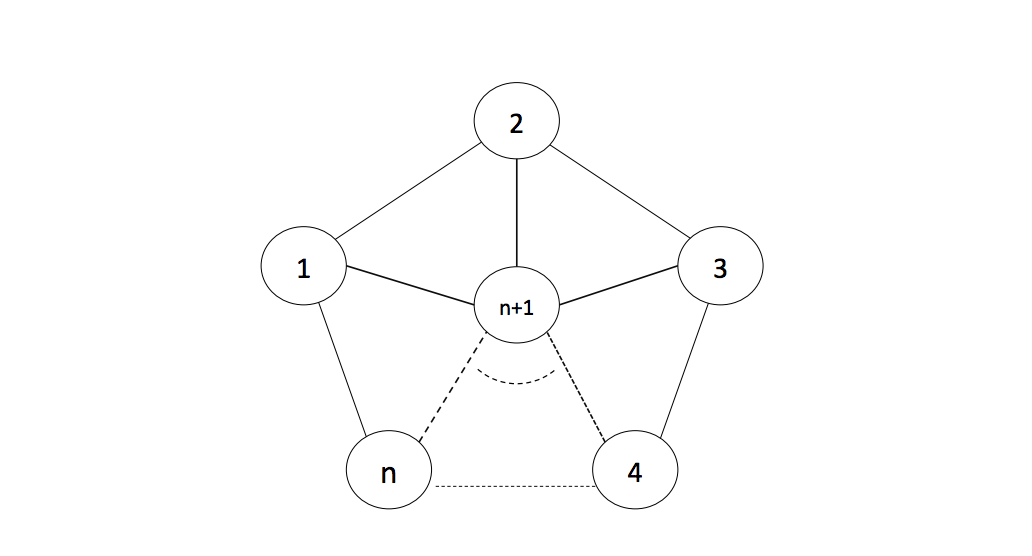
\includegraphics[width=10cm]{topo.png}
\linebreak
The total number of updates sent as a function of the number of routers in the topology is contained in the array: 
\linebreak

[16
23
33
45
56
68
81
95
110
126
143
161
180
200
221
243
266
290
315
341
368
396
425
455
486
518
551
585
620
656
693
731
770
810
851
893
936
980
1025
1071
1118
1166
1215
1265
1316
1368
1421
1475]
\linebreak

The plot of this data is shown below.
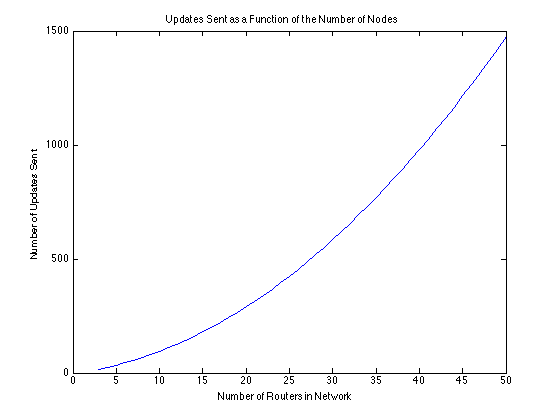
\includegraphics[width=13cm]{plot.png}
\linebreak
As we can see, with my RIPRouter implementation, the number of updates sent is relatively few and grows quadratically as the number of routers in the network grows. For a naive implementation, this is fantastic - our growth is not out of control and we are able to converge in a short amount of time. 
\end{center}
\end{document}